\documentclass[border=4pt]{standalone}
\usepackage{amsmath,amssymb,tikz}\usetikzlibrary{arrows.meta,calc}
\definecolor{figB}{RGB}{31,90,166}\definecolor{figR}{RGB}{176,48,48}\definecolor{figG}{RGB}{46,125,50}\definecolor{figO}{RGB}{214,120,20}
\begin{document}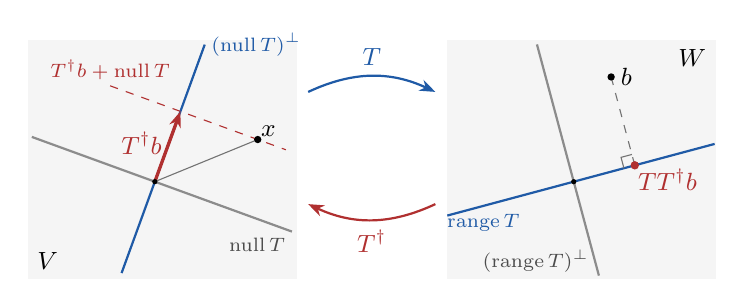
\begin{tikzpicture}[scale=0.95,>={Stealth[length=2mm]}]
% ---------- V ----------
\fill[black!4] (-1.7,-1.3) rectangle (1.9,1.9);
\node[font=\small,anchor=south west] at (-1.7,-1.3) {$V$};
\draw[thick,black!45] (160:1.75)--(-20:1.95) node[below left,font=\scriptsize,black!70,inner sep=2pt]{$\operatorname{null}T$};
\draw[thick,figB] (250:1.3)--(70:1.95) node[right,font=\scriptsize,inner sep=2pt]{$(\operatorname{null}T)^\perp$};
% least-squares solutions: T^dagger b + null T
\coordinate (Tb) at (70:1.0);
\draw[dashed,figR] ($(Tb)+(160:1.0)$) node[above,font=\scriptsize,inner sep=2pt]{$T^\dagger b+\operatorname{null}T$}--($(Tb)+(-20:1.5)$);
\coordinate (x) at ($(Tb)+(-20:1.1)$);
\draw[black!55] (0,0)--(x);
\fill (x) circle (1.4pt) node[above right,font=\small,inner sep=1pt]{$x$};
\draw[->,very thick,figR] (0,0)--(Tb) node[pos=0.55,left,font=\small,inner sep=2pt]{$T^\dagger b$};
\fill (0,0) circle (1pt);
% ---------- W ----------
\begin{scope}[xshift=5.6cm]
\fill[black!4] (-1.7,-1.3) rectangle (1.9,1.9);
\node[font=\small,anchor=north east] at (1.9,1.9) {$W$};
\draw[thick,black!45] (285:1.3)--(105:1.9);
\node[font=\scriptsize,black!70,left,inner sep=2pt] at (285:1.1) {$(\operatorname{range}T)^\perp$};
\draw[thick,figB] (195:1.75)--(15:1.95);
\node[font=\scriptsize,figB,below,inner sep=3pt] at (195:1.25) {$\operatorname{range}T$};
\coordinate (b) at (0.5,1.4); \coordinate (Pb) at (0.816,0.219);
\draw[dashed,black!55] (b)--(Pb);
\draw[black!55,thin] ($(Pb)+(15:-0.15)$)--++(105:0.15)--++(15:0.15);
\fill (b) circle (1.4pt) node[right,font=\small]{$b$};
\fill[figR] (Pb) circle (1.6pt) node[below right,font=\small,inner sep=1pt]{$TT^\dagger b$};
\fill (0,0) circle (1pt);
\end{scope}
% ---------- the maps ----------
\draw[->,thick,figB] (2.05,1.2) to[bend left=25] node[above,font=\small]{$T$} (3.75,1.2);
\draw[->,thick,figR] (3.75,-0.3) to[bend left=25] node[below,font=\small]{$T^\dagger$} (2.05,-0.3);
\end{tikzpicture}\end{document}
